\section{Evaluating the impact of real rain}
\label{sec:real_data}

\begin{figure*}[!t] 
 \centering
 \scriptsize
 \setlength{\tabcolsep}{0.001\linewidth}
 \renewcommand{\arraystretch}{1.25}
 \begin{tabular}{cccccc}
  \multirow{1}{*}[1.15cm]{\rotatebox{90}{Input}} & 
 
\includegraphics[width=0.222\linewidth]{figures/results/real_rain/rain/000000.jpg} &
 
\includegraphics[width=0.222\linewidth]{figures/results/real_rain/rain/000145.jpg} &
 
\includegraphics[width=0.222\linewidth]{figures/results/real_rain/rain/002346.jpg} & 
 
\includegraphics[width=0.222\linewidth]{figures/results/real_rain/rain/004978.jpg} \\
 
  \multirow{1}{*}[1.5cm]{\rotatebox{90}{YOLOv2} \rotatebox{90}{~~~\cite{redmon2017yolo9000}} } & 
 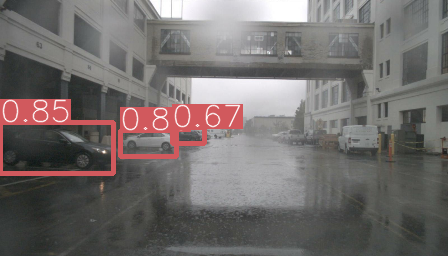
\includegraphics[width=0.222\linewidth]{figures/results/real_rain/yolov2/000000.png} &
 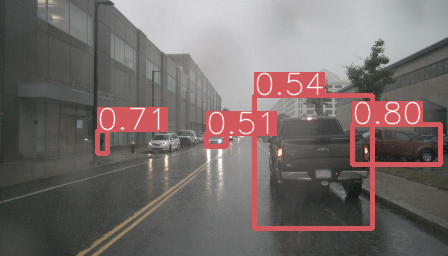
\includegraphics[width=0.222\linewidth]{figures/results/real_rain/yolov2/000145.png} &
 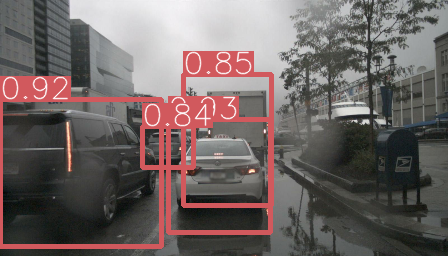
\includegraphics[width=0.222\linewidth]{figures/results/real_rain/yolov2/002346.png} & 
 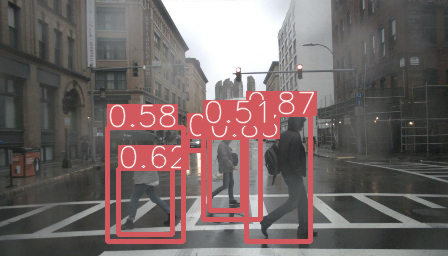
\includegraphics[width=0.222\linewidth]{figures/results/real_rain/yolov2/004978.png} \\
 
  \multirow{1}{*}[1.35cm]{\rotatebox{90}{PSPNet} \rotatebox{90}{~~~\cite{zhao2017pspnet}} } &
 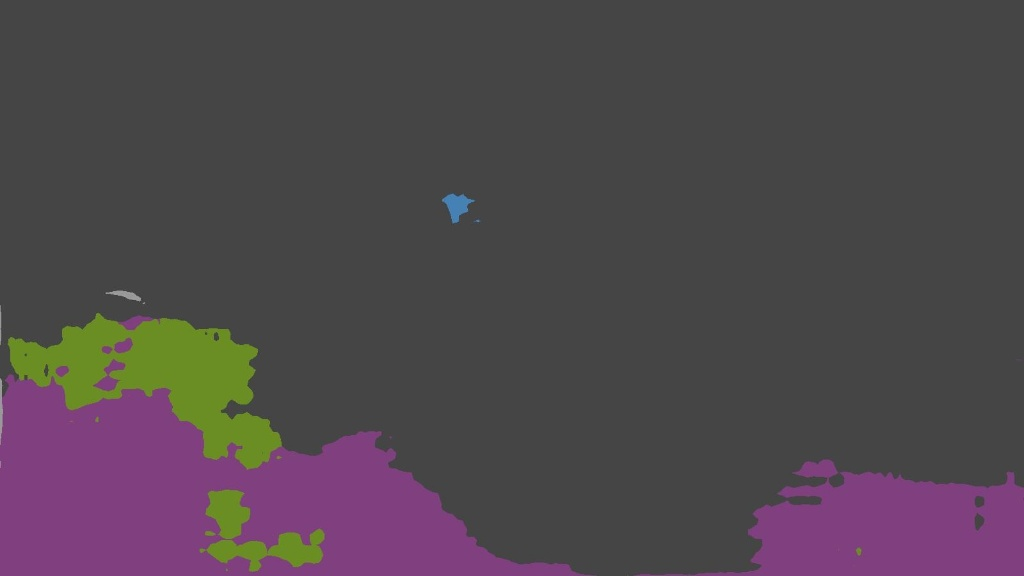
\includegraphics[width=0.222\linewidth]{figures/results/real_rain/pspnet/000000_color_lr.jpg} &
 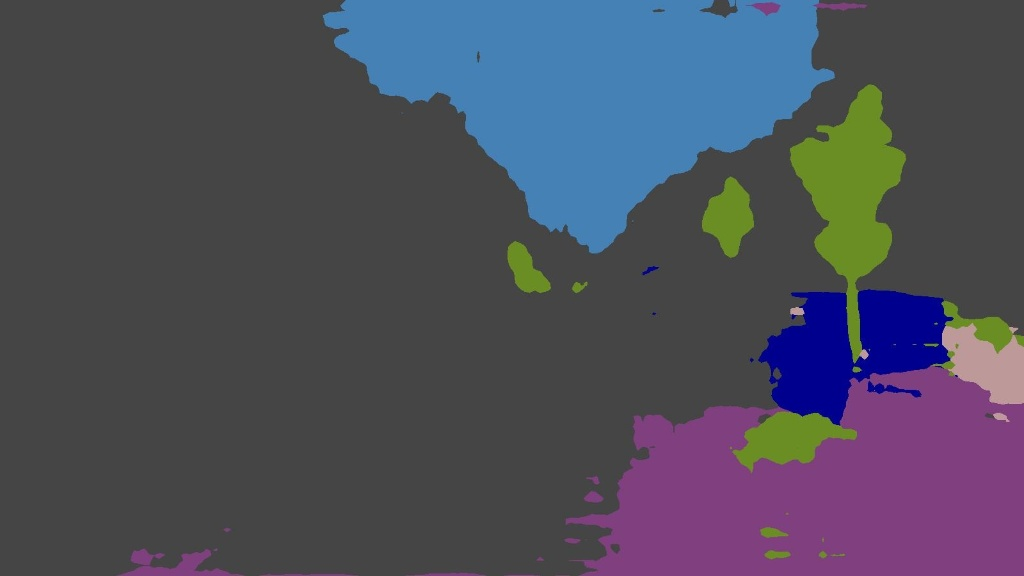
\includegraphics[width=0.222\linewidth]{figures/results/real_rain/pspnet/000145_color_lr.jpg} &
 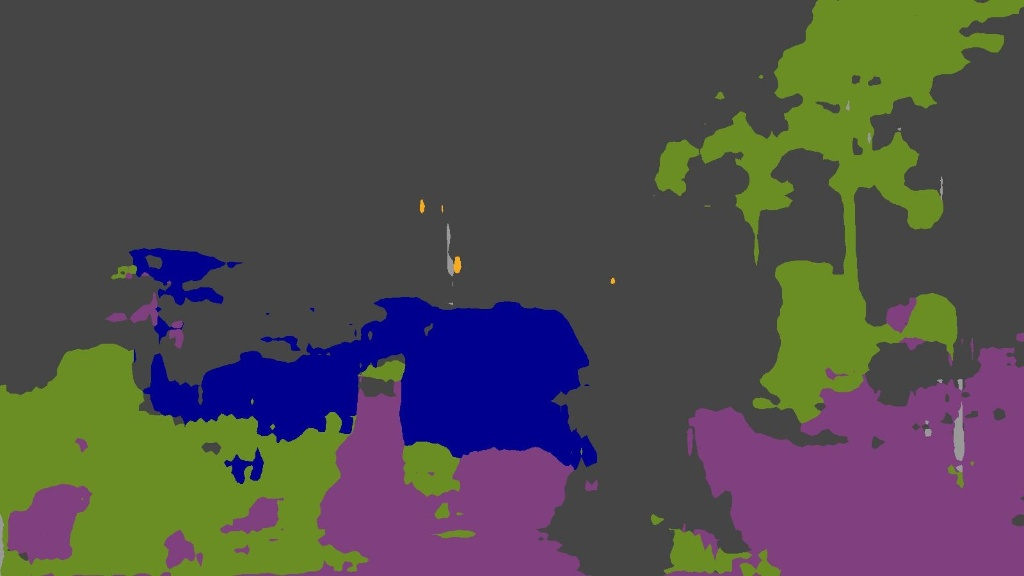
\includegraphics[width=0.222\linewidth]{figures/results/real_rain/pspnet/002346_color_lr.jpg} & 
 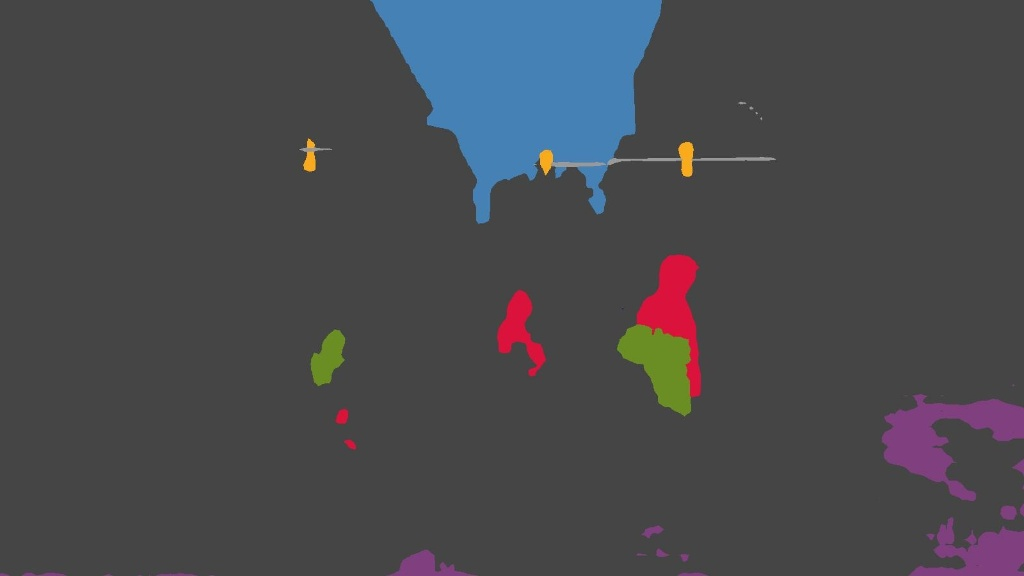
\includegraphics[width=0.222\linewidth]{figures/results/real_rain/pspnet/004978_color_lr.jpg} \\

  \multirow{1}{*}[1.625cm]{\rotatebox{90}{Monodepth2} \rotatebox{90}{~~~~~~\cite{godard2019digging}} } & 
 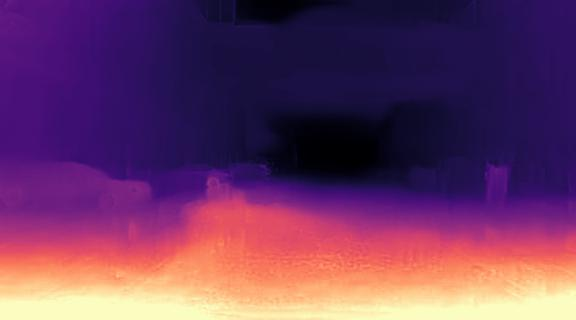
\includegraphics[width=0.222\linewidth]{figures/results/real_rain/monodepth2/000000.jpg} &
 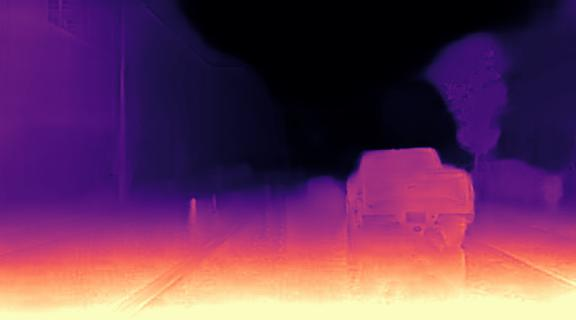
\includegraphics[width=0.222\linewidth]{figures/results/real_rain/monodepth2/000145.jpg} &
 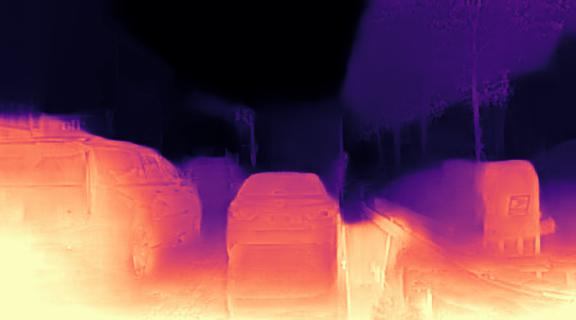
\includegraphics[width=0.222\linewidth]{figures/results/real_rain/monodepth2/002346.jpg} & 
 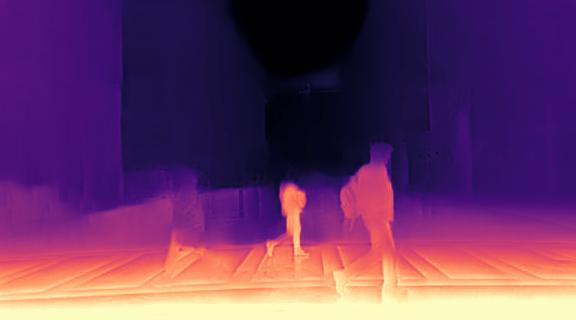
\includegraphics[width=0.222\linewidth]{figures/results/real_rain/monodepth2/004978.jpg} \\
 \end{tabular}
 \caption{\textbf{Qualitative results on real rainy images from the nuScenes dataset.} Shown for different tasks: object detection (top line), semantic segmentation (middle line), and depth estimation (bottom line) } %
 \label{fig:eval_qualitative_real_rain}
\end{figure*}

We now aim at quantifying the impact of rain on three computer vision tasks: object detection, semantic segmentation, and depth estimation. These tasks are critical for any outdoor vision systems such as mobile robotics, autonomous driving, or surveillance. Before we experiment on rain-augmented images with our PBR, GAN, and GAN+PBR approaches, we first experiment on real rainy photographs. 

For this, we use the nuScenes dataset~\cite{caesar2019nuscenes}. Benefiting from coarse frame-wise weather annotations in the dataset, we split nuScenes images\footnote{Note that only front camera and annotated key frames are used for consistency and ground truth accuracy.} in two subsets: ``nuScenes-clear'' (images without rain) and ``nuScenes-rain'' (rainy images). Due to the noisy weather labels, we cross-validated each frame with a historic weather database\footnote{Weather database at \url{https://openweathermap.org}.} using GPS location and time, and only kept frames where the nuScenes label agreed with the weather database. This resulted in sets of 24134 images for nuScenes-clear, and 6028 for nuScenes-rain. In this dataset, rain images are dark, gloomy, the sky is heavily covered, and no falling rain is visible but there are unfocused raindrops occlusions on the lens.

We experiment on these sets of real images with algorithms from each task: YOLOv2~\cite{redmon2017yolo9000} for object detection, PSPNet~\cite{zhao2017pspnet} for semantic segmentation, and Monodepth2~\cite{godard2019digging} for depth estimation. The nuScenes-clear set is split into train/test subsets of 19685/4449 images from 491/110 scenes. The nuScenes-rain is also split into train/test subsets of 5419/609 images from 134/15 scenes. Here, 1000 images from the nuScenes-clear(test) and all images from the nuScenes-rain(test) subset are used for evaluation (train will be used for the GAN in sec.~\ref{sec:rain_setup}). These training and testing sets and subsets are all displayed in table \ref{tab:splits} in appendix~\ref{sec:app-data-splits}. Note that a large number of images were needed to train the CycleGAN for image translation and, to avoid any overlap in image sequences, it unfortunately left a relatively small subset of nuScenes for the evaluation on real rainy images.

For object detection and depth estimation, we first pre-train each algorithm on ImageNet (Darknet53, $448\times448$) and KITTI (monocular, $1024\times320$) respectively, and further finetune them on the nuScenes-clear(train) subset to limit the domain gap between datasets. We then evaluate their performance on the aforementioned test subsets. For segmentation, since semantic labels are not provided on nuScenes, we carefully annotated 25 images from both nuScenes-clear(test) and nuScenes-rain(test). Since we do not have enough labeled data for finetuning, we use our model pretrained on Cityscapes~\cite{Cordts2016Cityscapes}, with the caveat that there may be a significative domain gap between training and evaluation. 

Table~\ref{fig:real_rain_perf} reports the results of this experiment. The performance on real rainy images compared to clear images for all three tasks are a mAP of 16.30\% instead of 32.53\% for object detection, an AP of 18.7\% instead of 40.8\% for semantic segmentation and a square relative error of 3.53\% instead of 2.96\% for depth estimation. Corresponding qualitative results are displayed in fig.~\ref{fig:eval_qualitative_real_rain}. 
As expected, real rain deteriorates the performance of all algorithms on all tasks. However, we cannot evaluate how rain \emph{intensity} affects these algorithms since it would require the accurate measurement of the rainfall rate at the time of capture.


\begin{table}
 \centering
  \scriptsize
  \setlength{\tabcolsep}{0.18cm}
  \renewcommand{\arraystretch}{1.0}
  \begin{tabular}{llcc}
   \toprule
   Tasks & Metric & Clear & Rain \\
   \midrule
   Object detection~\cite{redmon2017yolo9000} & mAP (\%) $\uparrow$ & 24.70 & 11.09 \\
   Semantic segmentation~\cite{zhao2017pspnet} & AP (\%) $\uparrow$ & 40.8 & 18.7 \\
   Depth estimation~\cite{godard2019digging} & Sq. err. (\%) $\downarrow$ & 2.96 & 3.53 \\ 
   \bottomrule
 \end{tabular}\hspace{.025\linewidth}
 \caption{\textbf{Vision tasks on real clear/rain images from nuScenes~\cite{caesar2019nuscenes}.} Significant performance drops are observed in rainy weather.}
 \label{fig:real_rain_perf}
\end{table} 
